\documentclass[a4paper,10pt]{article}
\usepackage{graphicx}
\usepackage{amsmath}
\usepackage{hyperref}
\usepackage{geometry}
\usepackage{caption}
\usepackage{subcaption}
\usepackage{booktabs}
\usepackage{color}
\usepackage{listings}
\definecolor{GrayCodeBlock}{RGB}{241,241,241}
\definecolor{BlackText}{RGB}{110,107,94}
\definecolor{RedTypename}{RGB}{182,86,17}
\definecolor{GreenString}{RGB}{96,172,57}
\definecolor{PurpleKeyword}{RGB}{184,84,212}
\definecolor{GrayComment}{RGB}{170,170,170}
\definecolor{GoldDocumentation}{RGB}{180,165,45}
\lstdefinelanguage{rust}
{
    columns=fullflexible,
    keepspaces=true,
    frame=single,
    framesep=0pt,
    framerule=0pt,
    framexleftmargin=4pt,
    framexrightmargin=4pt,
    framextopmargin=5pt,
    framexbottommargin=3pt,
    xleftmargin=4pt,
    xrightmargin=4pt,
%    backgroundcolor=\color{GrayCodeBlock},
    basicstyle=\ttfamily\color{BlackText},
    keywords={
        true,false,
        unsafe,async,await,move,
        use,pub,crate,super,self,mod,
        struct,enum,fn,const,static,let,mut,ref,type,impl,dyn,trait,where,as,
        break,continue,if,else,while,for,loop,match,return,yield,in
    },
    keywordstyle=\color{PurpleKeyword},
    ndkeywords={
        bool,u8,u16,u32,u64,u128,i8,i16,i32,i64,i128,char,str,
        Self,Option,Some,None,Result,Ok,Err,String,Box,Vec,Rc,Arc,Cell,RefCell,HashMap,BTreeMap,
        macro_rules
    },
    ndkeywordstyle=\color{RedTypename},
    comment=[l][\color{GrayComment}\slshape]{//},
    morecomment=[s][\color{GrayComment}\slshape]{/*}{*/},
    morecomment=[l][\color{GoldDocumentation}\slshape]{///},
    morecomment=[s][\color{GoldDocumentation}\slshape]{/*!}{*/},
    morecomment=[l][\color{GoldDocumentation}\slshape]{//!},
    morecomment=[s][\color{RedTypename}]{\#![}{]},
    morecomment=[s][\color{RedTypename}]{\#[}{]},
    stringstyle=\color{GreenString},
    string=[b]"
}


\geometry{margin=1in}

\title{
  Branch-prediction effects in quick sort \\
\small Quick sort with and without branching in the partitioning function}
\author{Max Boone (s2081318)}
\date{\today}

\begin{document}

\maketitle

\section{Introduction}

This report briefly describes and benchmarks two implementations of
quicksort, one implementation that uses an branching if-statement in
its partitioning function and one that uses an assigned conditional
to avoid branch misses. First, the implementation of the sorting
algorithm is discussed. Then, performance results of sorting are
provided. Finally, the results are concluded.

\section{Implementation}

The quicksort algorithm can be divided into two steps. First, the sorting
algorithm calls a partitioning function that separates the list into a partition
with the smallest and partition with the largest numbers. A pivot index shows
where the partitions are split. Second, the sorting algorithm is called recursively
on the left and right constituents and sorts them independently.

In the partitioning function, a conditional swapping is done based on
if the element is smaller than the chosen pivot. Due to the randomness
of this operation the branch predictor is likely to mispredict whether
to jump or not to the swapping instruction. As an optimization, this is
replaced by a conditional assignment and a temporary variable, to avoid
having to jump to another instruction. The main difference between the
functions is shown in Listing 1.

\begin{lstlisting}[language=rust, caption={Both partitioning implementations in Rust}, captionpos=b]
/// Branchless implementation
for j in 0..high {
    let c = list[j] <= list[high];
    let t = list[i];
    list[i] = list[j] * c as u32 + t * (1 - c as u32);
    list[j] = t * c as u32 + list[j] * (1 - c as u32);
    i += c as usize;
}

/// Branching implementation
for j in 0..high {
    if list[j] <= list[high] {
        list.swap(i, j);
        i += 1;
    }
}
\end{lstlisting}

In the final compiled instructions for the branchless implementation the 
first two list accesses get a branching instruction to check for out-of-bounds
access. However, as in-bounds access is certain, the branch predictor will not
suffer here. Then, the conditional is calculated and the swapping is implemented
with conditional-move instructions.

The branching implementation is compiled in fewer instructions, it also does the
out-of-bounds checks, but jumps to the swapping and increasing instructions if the
condition evaluates to true. If the result of the condition is random, the branch
predictor will have branch misses here.

\section{Performance}

The system used for the benchmarks is a Surface Pro X SQ2 device 
with an Kryo-4XX-Gold ARMv8 SoC and 16 GiB of LPDDR4 4266 MHz RAM.

Each sorting run gets one warm-up run to get the file contents loaded
and cached into memory. Even though only the sorting time is counted, a
difference between a cold and warm run was observed during testing.
Only warm runs are used in the results. The runtime is measured in the
application by timings around the highest call of the sort function.
A branch miss counter from the Linux \texttt{perf} API is used in around
the sort function.

\begin{table}[h!]
    \centering
    \caption{Speedup (Branching Time / Branchless Time)}
    \label{tab:speedup_descriptive}
    \begin{tabular}{ccccccc}
        \toprule
        Mean & Std Dev & Min & 25\% & Median (50\%) & 75\% & Max \\
        \midrule
        1.429 & 0.544 & 0.819 & 1.097 & 1.128 & 1.736 & 3.876 \\
        \bottomrule
    \end{tabular}
\end{table}

In Figure 1 we see the runtimes of both implementations next to eachother. The branchless
implementation on the right is generally faster with a speedup of 1.42 on average, further
descriptives given in Table 1.
In Figure 2 we see the branch misses of both implementations, as expected, the branching 
implementation has many more branch misses than the branchless implementation. Furthermore,
the branch misses occur more on datasets that are (more) randomly distributed.

\begin{figure}[htbp]
    \centering
    % First graph
    \begin{subfigure}[b]{0.40\textwidth}
        \centering
        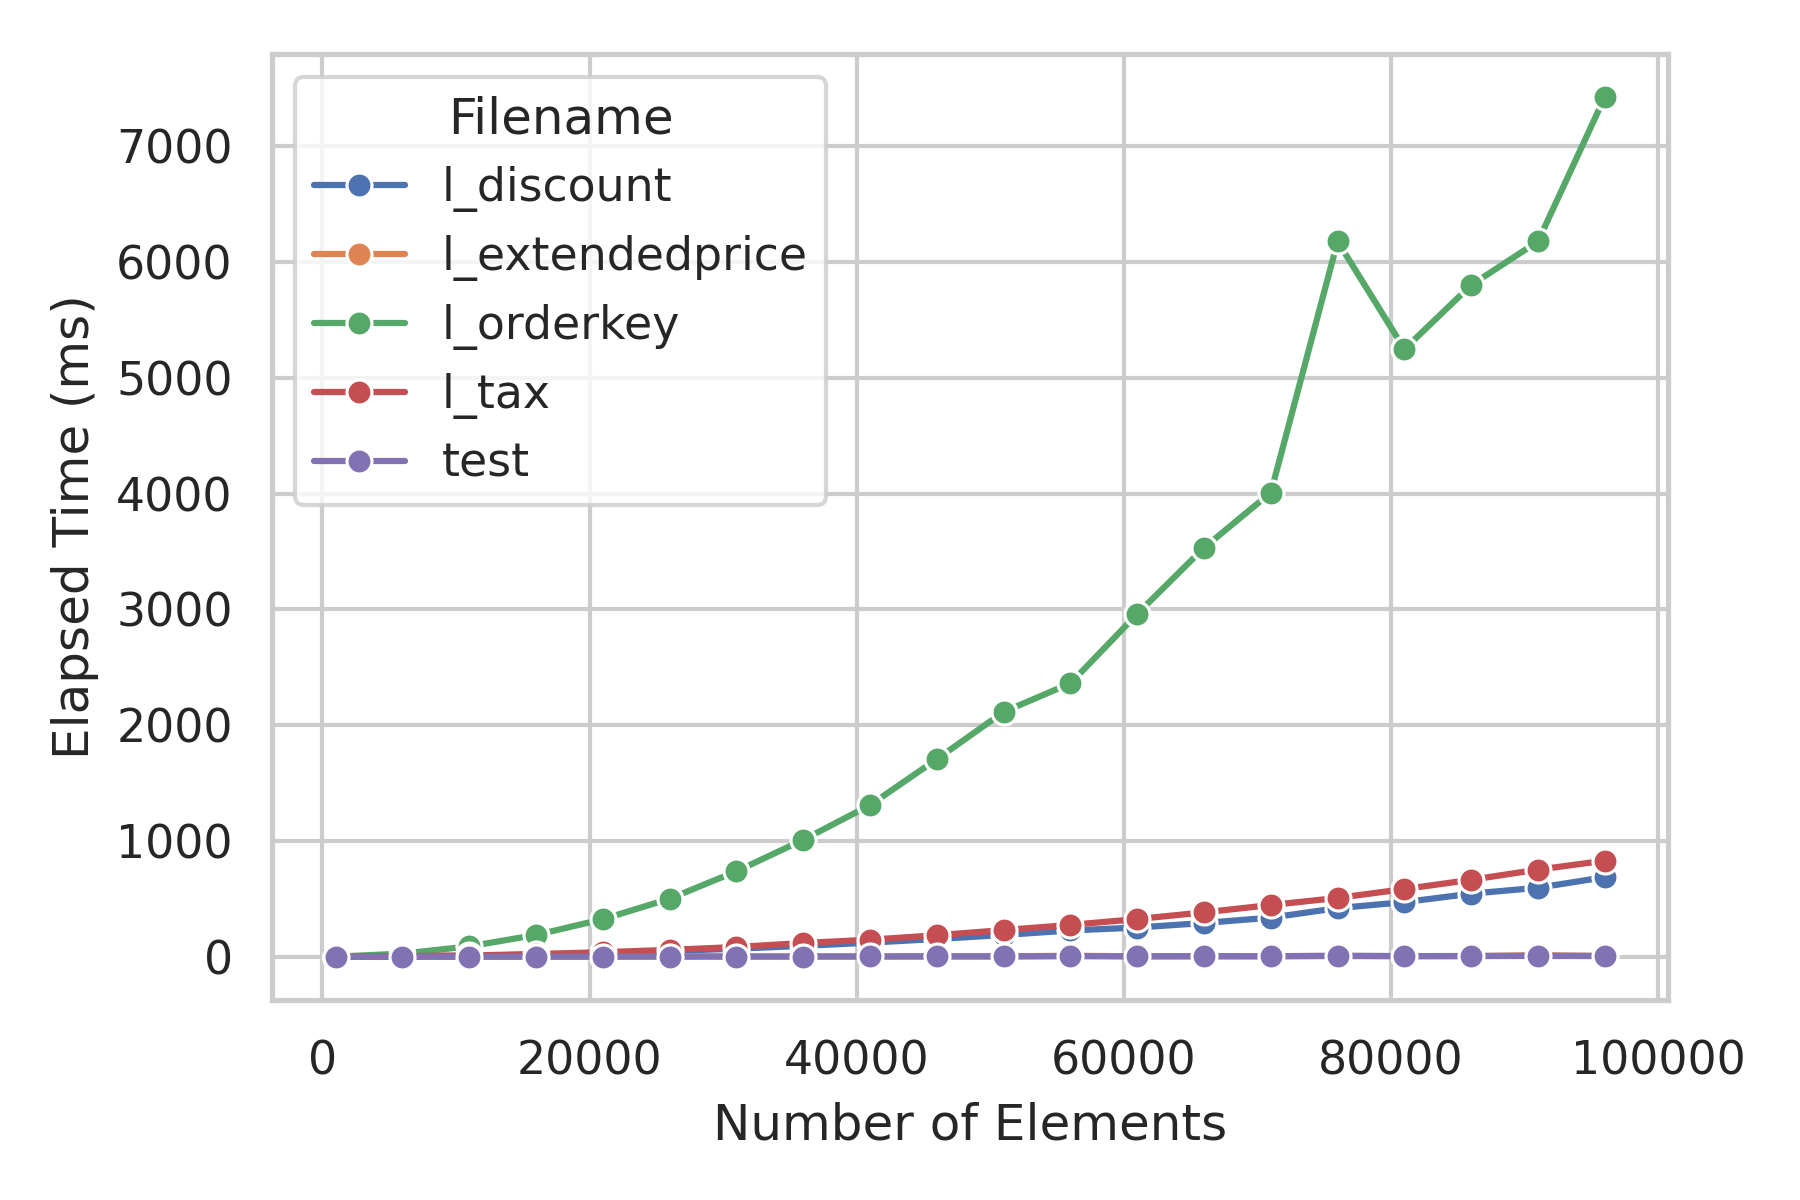
\includegraphics[width=\textwidth]{../graphs/branching_elapsed.png}
        \caption{Branching}
        \label{fig:elapsed_branching}
    \end{subfigure}
    % Second graph
    \begin{subfigure}[b]{0.40\textwidth}
        \centering
        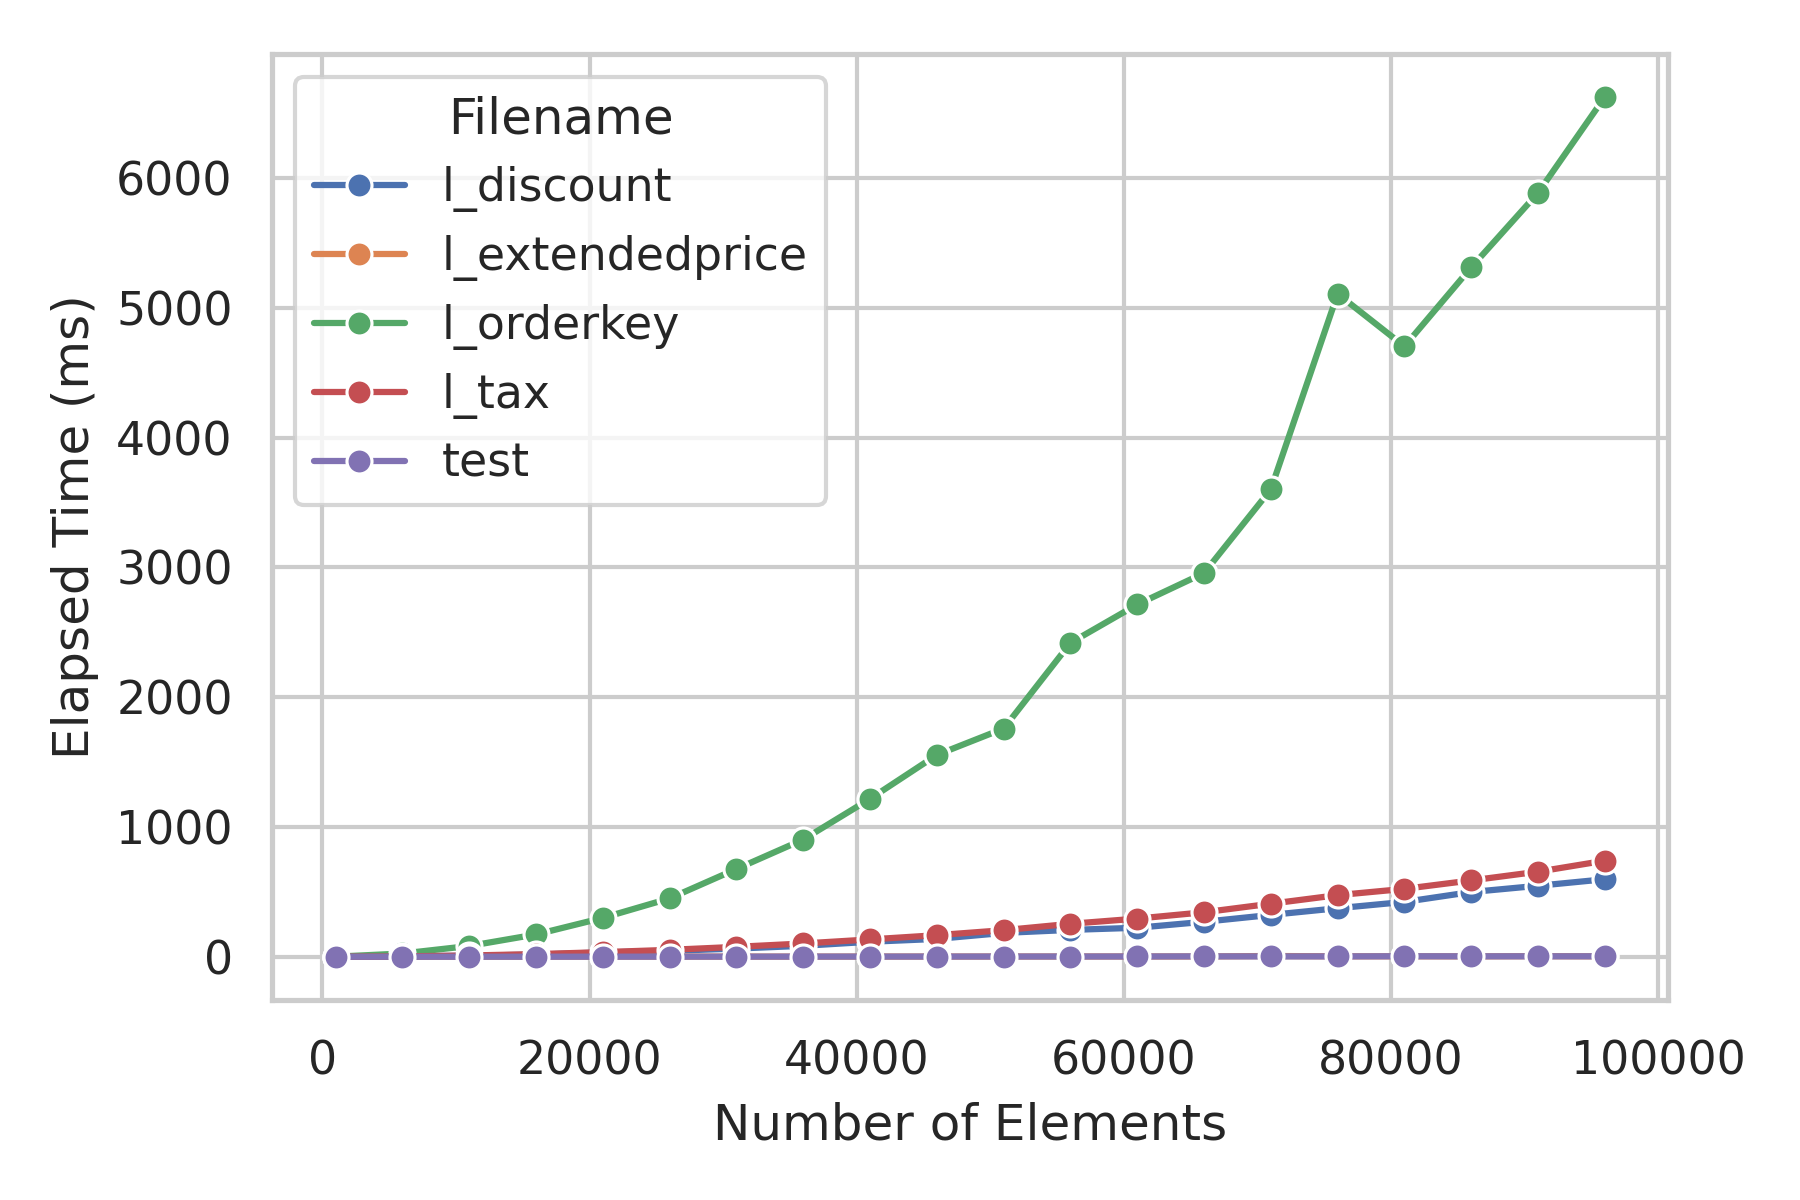
\includegraphics[width=\textwidth]{../graphs/condition-assign_elapsed.png}
        \caption{Branchless}
        \label{fig:elapsed_branchless}
    \end{subfigure}
    \caption{Elapsed time to sort datasets.}
    \label{fig:elapsed_time}
\end{figure}

\begin{figure}[htbp]
    \centering
    % First graph
    \begin{subfigure}[b]{0.40\textwidth}
        \centering
        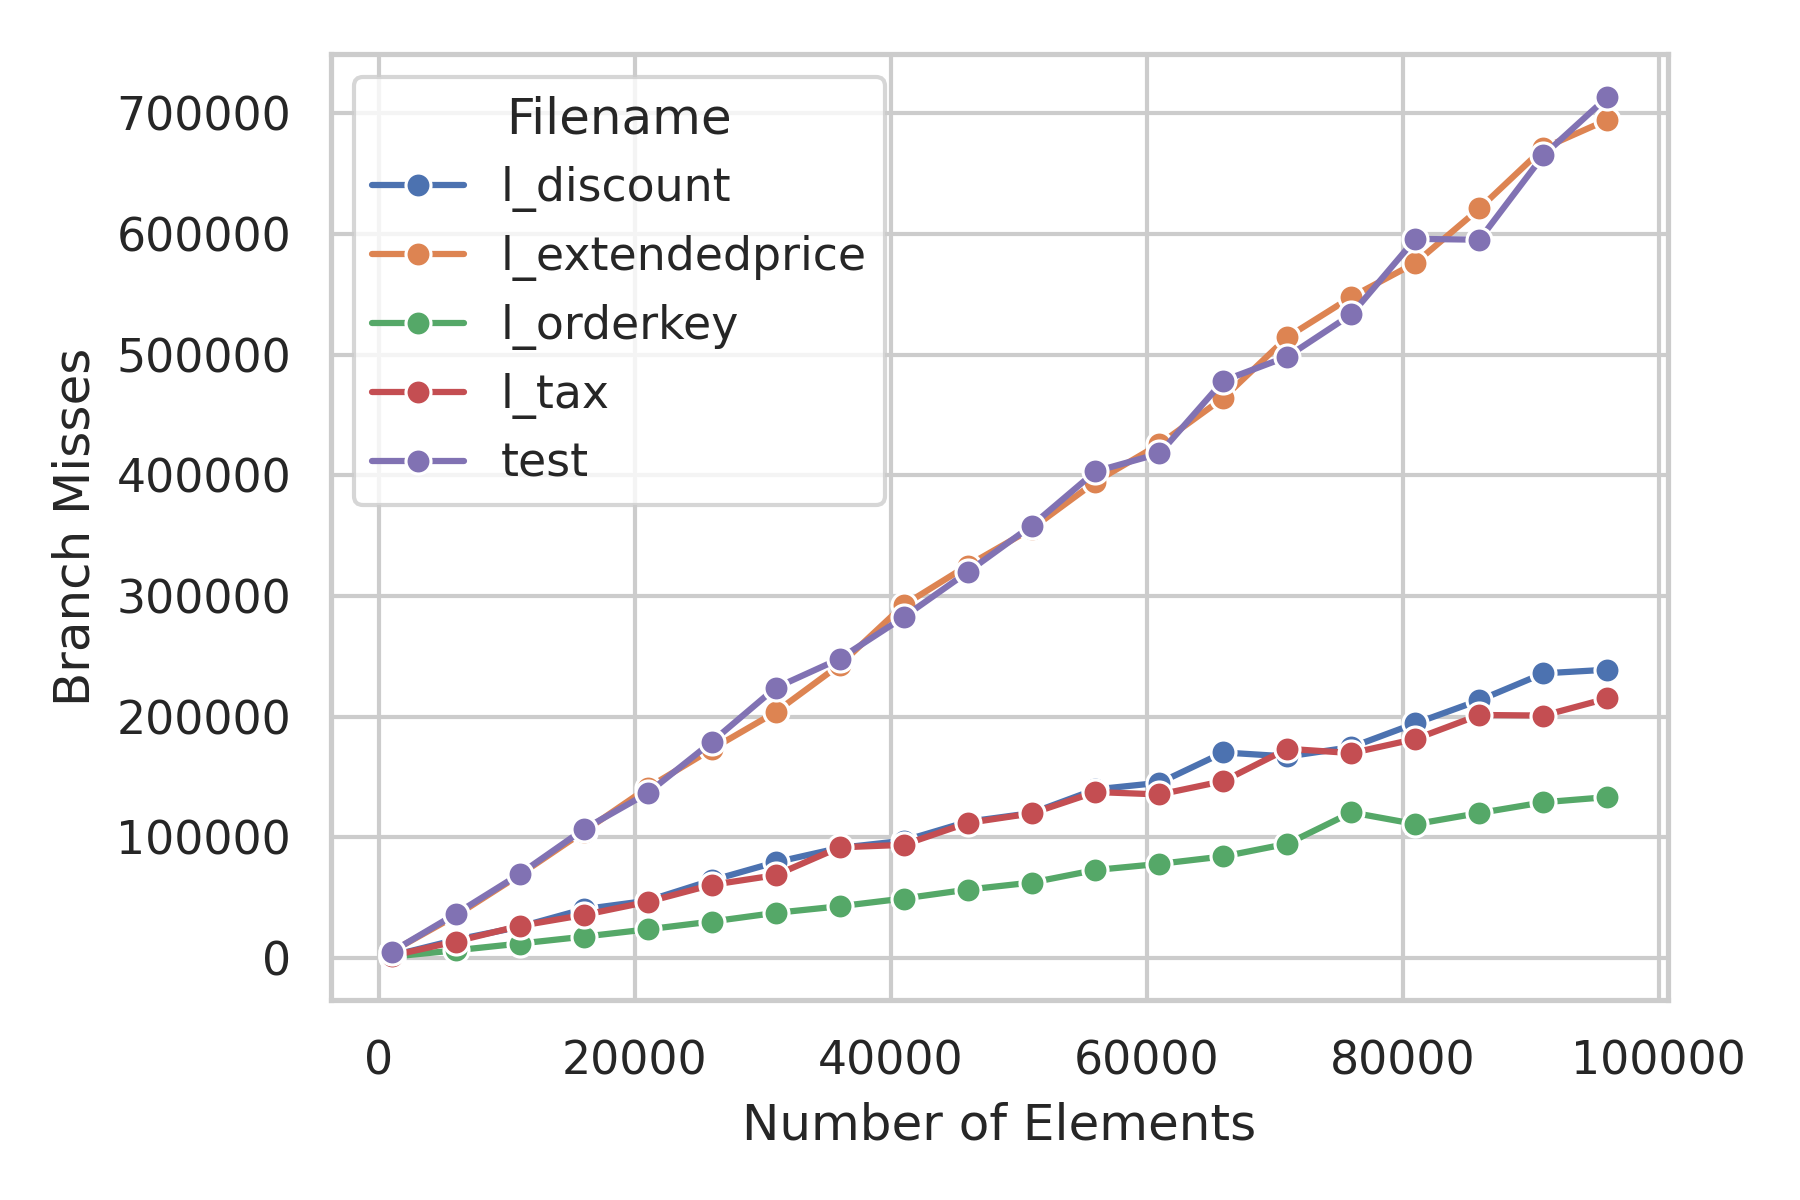
\includegraphics[width=\textwidth]{../graphs/branching_misses.png}
        \caption{Branching}
        \label{fig:misses_branching}
    \end{subfigure}
    % Second graph
    \begin{subfigure}[b]{0.40\textwidth}
        \centering
        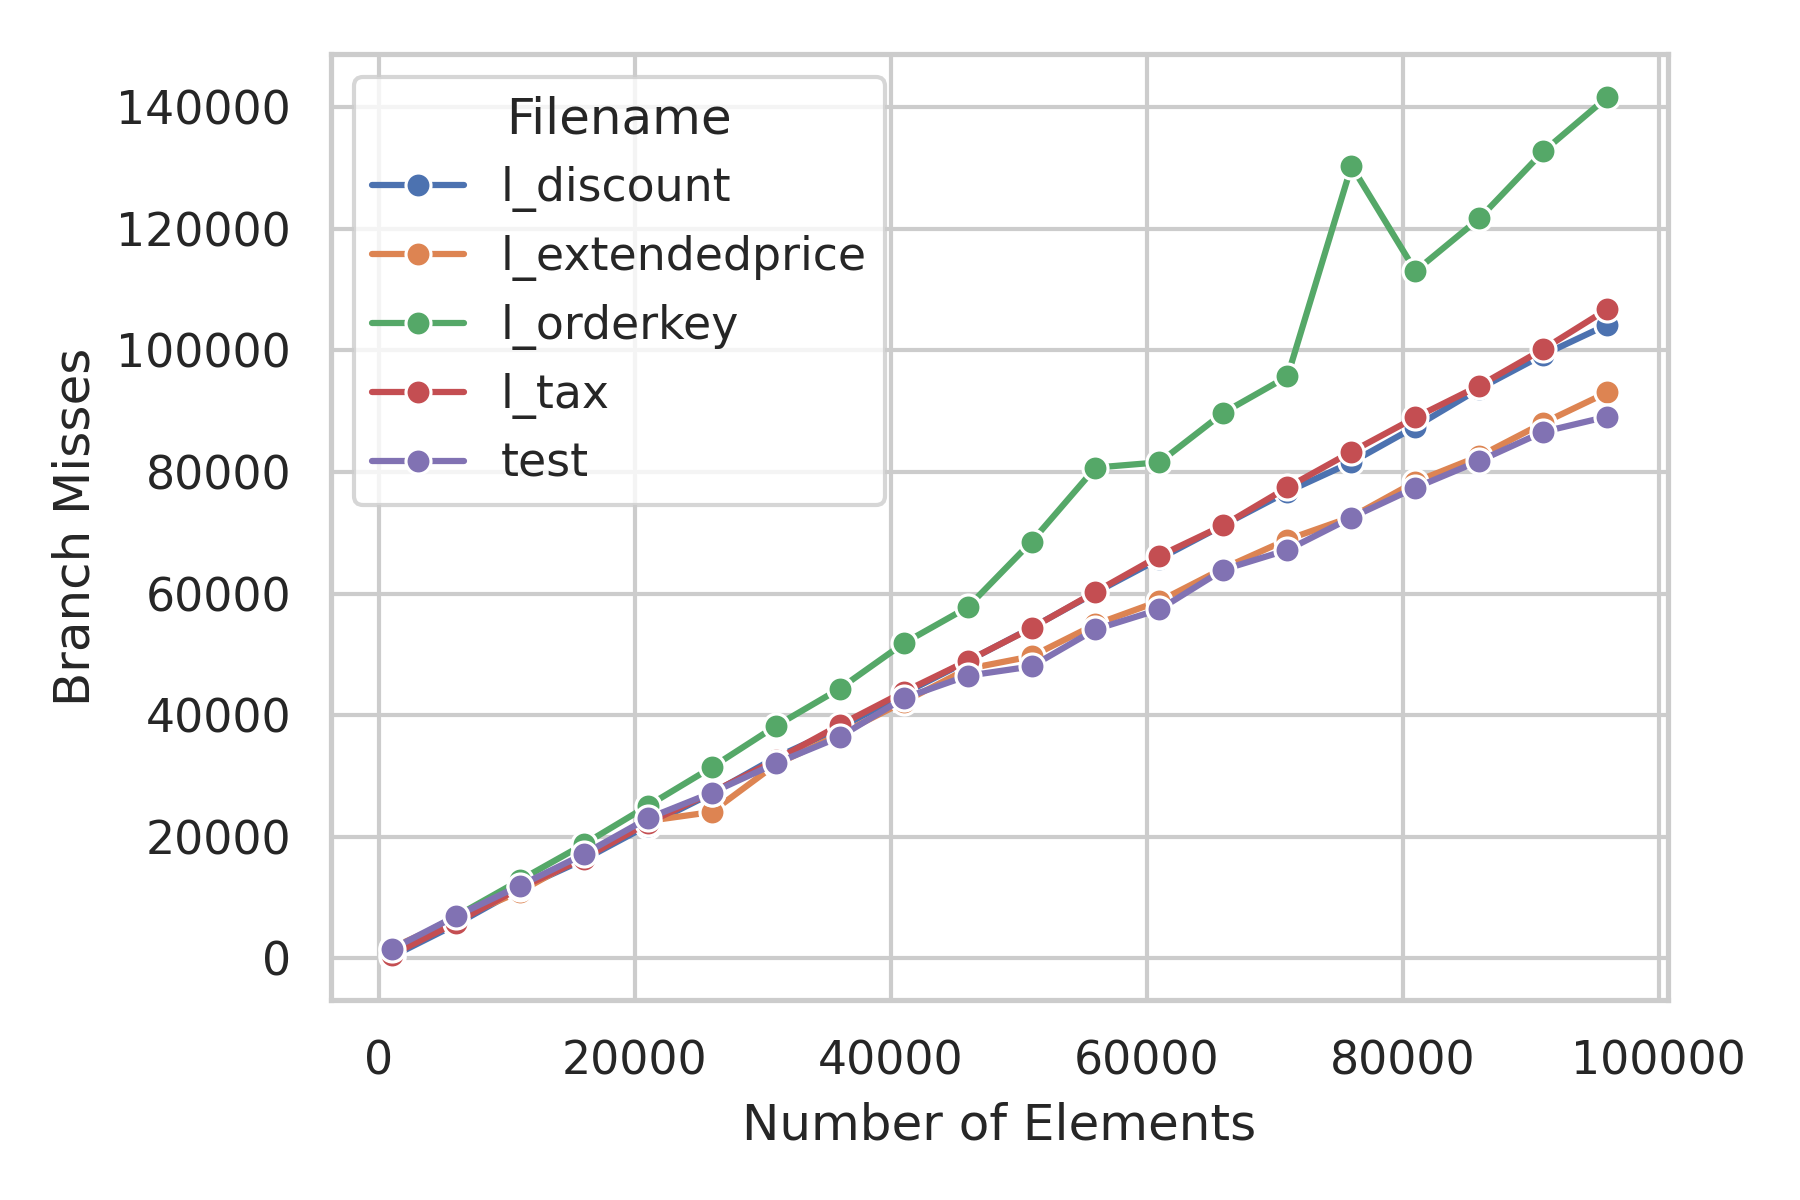
\includegraphics[width=\textwidth]{../graphs/condition-assign_misses.png}
        \caption{Branchless}
        \label{fig:misses_branchless}
    \end{subfigure}
    \caption{Branch misses in sorting function.}
    \label{fig:elapsed_time}
\end{figure}

\section{Conclusion}

The speedup of the branchless implementation is not as large as initially expected. 
This might be due to the architecture of 
the used processor, or due to the compiler inserting branching instructions to check for
out-of-bounds access. Nevertheless, the experiments confirm that the branch mispredictions
are mitigated using the branchless implementation.

\end{document}
